\documentclass[12pt]{article}
\usepackage{ctex}
\usepackage[english]{babel}
\usepackage{blindtext}
\usepackage{nameref}
\usepackage{fancyhdr}
\usepackage{amsmath,amssymb,amsthm}
\usepackage{graphicx,float}
\usepackage{physics}
\usepackage{pgfplots}
\usepackage[a4paper, total={6in, 9in}]{geometry}

\graphicspath{{../picture/}}

\pagestyle{fancy}
\fancyhf{}
\fancyhf[HL]{F4 第五級 M2 模擬試題}
\fancyhf[HR]{限時:1小時30分鐘}
\fancyhf[CF]{\thepage}

\newcommand{\innerprod}[2]{\langle{#1},{#2}\rangle}
\newcommand{\id}{\mathtt{id}}

\newtheorem*{definition}{Definition}
\newtheorem*{theorem}{Theorem}
\newtheorem*{corollary}{Corollary}
\newtheorem*{lemma}{Lemma}
\newtheorem*{proposition}{Proposition}
\newtheorem*{remark}{Remark}
\newtheorem*{claim}{Claim}
\newtheorem*{example}{Example}
\newtheorem*{axiom}{Axiom}

\begin{document}
    \thispagestyle{plain}

    \centering 

    \section*{練習試卷\\數學延伸單元\\單元2 (代數與微積分)\\試題-答題簿}

    限時: 1.5 小時

    姓名:\hrulefill \hfill 得分:\hrulefill/100

    學校:\hrulefill

    \raggedright

    \subsection*{規則}

    \begin{enumerate}
        \item 此試卷必須使用中文回答。
        \item 除特別指明外,需詳細列出所有算式。
        \item 除特別指明外,數值答案必須用真確值表示。
        \item 本試卷只作\textbf{内部使用}。
        \item 所有試題取自AL/CE/DSE歷届試題,來源: https://www.dse.life/ppindex/m2/
    \end{enumerate}

    \newpage
    \begin{enumerate}
        \item (1997-CE-A MATH 2 \#07(Modified)) 設對於任意正整數$n$,$T_n=(n^2+1)(n!)$。運用數學歸納法,證明對於所有正整數$n$, $$\sum_{k=1}^{n}T_k=n[(n+1)!]$$\hfill(6 分)
        
            \hrulefill
            
            \hrulefill
            
            \hrulefill
            
            \hrulefill
            
            \hrulefill
            
            \hrulefill
            
            \hrulefill
            
            \hrulefill
            
            \hrulefill
            
            \hrulefill
            
            \hrulefill
            
            \hrulefill
            
            \hrulefill
            
            \hrulefill
            
            \hrulefill
            
            \hrulefill
            
            \hrulefill
            
            \hrulefill
            
            \hrulefill
            
            \hrulefill
            
            \hrulefill
            
            \hrulefill
            
            \hrulefill

        \pagebreak
        \item (1988-HL-GEN MATHS \#07(Modified)) 設 $$A_n=1^2-2^2+3^2-4^2+\dots+(-1)^{n-1}n^2$$ 及 $$B_n=1+2+3+\dots+n=\frac{n(n+1)}{2}$$ 其中 $n$ 為正整數。\begin{enumerate}
            \item 運用數學歸納法,證明對於所有正整數$n$, $A_n=(-1)^{n-1}B_n$。
            \item 由此,或以其他方式,求 $\displaystyle\sum_{n=1}^{2m}A_n$及 $\displaystyle\sum_{n=1}^{2m+1}A_n$的值。
        \end{enumerate}\hfill(8分)
        
            \hrulefill
            
            \hrulefill
            
            \hrulefill
            
            \hrulefill
            
            \hrulefill
            
            \hrulefill
            
            \hrulefill
            
            \hrulefill
            
            \hrulefill
            
            \hrulefill
            
            \hrulefill
            
            \hrulefill
            
            \hrulefill
            
            \hrulefill
            
            \hrulefill
            
            \hrulefill
            
            \hrulefill
            
            \hrulefill
            
            \hrulefill
            
            \hrulefill
            
            \hrulefill
            
            \hrulefill
            
            \hrulefill
            
            \hrulefill
            
            \hrulefill
            
            \hrulefill
            
            \hrulefill
            
            \hrulefill
            
            \hrulefill
            
            \hrulefill
            
            \hrulefill
            
            \hrulefill
            
            \hrulefill
            
            \hrulefill
            
            \hrulefill
            
            \hrulefill
            
            \hrulefill
            
            \hrulefill
            
            \hrulefill
            
            \hrulefill
            
            \hrulefill
            
            \hrulefill
            
            \hrulefill
            
            \hrulefill
            
            \hrulefill
            
            \hrulefill

        \pagebreak
        \item (2017-DSE-MATH-EP(M2) \#02) 設 $\displaystyle (1+ax)^8=\sum_{k=0}^8 \lambda_k x^k$ 及 $\displaystyle(b+x)^9=\sum_{k=0}^9 \mu_k x^k$,其中$a$ 及$b$ 為常數。 已知 $\lambda_2:\mu_7=7:4$ 及 $\lambda_1+\mu_8+6=0$。求 $a$。\hfill(6分)
        
        \hrulefill
            
        \hrulefill
        
        \hrulefill
        
        \hrulefill
        
        \hrulefill
        
        \hrulefill
        
        \hrulefill
        
        \hrulefill
        
        \hrulefill
        
        \hrulefill
        
        \hrulefill
        
        \hrulefill
        
        \hrulefill
        
        \hrulefill
        
        \hrulefill
        
        \hrulefill
        
        \hrulefill
        
        \hrulefill
        
        \hrulefill
        
        \hrulefill
        
        \hrulefill
        
        \hrulefill
        
        \hrulefill
        
        \hrulefill

    \pagebreak
        \item (1989-HL-GEN MATHS \#05(Modified))  \begin{enumerate}
            \item 解方程 $\sin{x}-\sin{2x}+\sin{3x}=0$,其中 $0<x<2\pi$.
            \item 設 $f(\theta)=\sin{2\theta}+\sin{\theta}+\cos{\theta}$。\begin{enumerate}
                \item 試以$p$表示$f(\theta)$,其中 $p=\sin{\theta}+\cos{\theta}$。
                \item 利用 (i) 的結果及配方法, 求 $f(\theta)$的最小值。對於$0<\theta<\pi$,求 $\theta$ 的值使得 $f(\theta)$ 到達最小值。
            \end{enumerate}
        \end{enumerate}\hfill(18分)

        \hrulefill
            
            \hrulefill
            
            \hrulefill
            
            \hrulefill
            
            \hrulefill
            
            \hrulefill
            
            \hrulefill
            
            \hrulefill
            
            \hrulefill
            
            \hrulefill
            
            \hrulefill
            
            \hrulefill
            
            \hrulefill
            
            \hrulefill
            
            \hrulefill
            
            \hrulefill
            
            \hrulefill
            
            \hrulefill
            
            \hrulefill
            
            \hrulefill
            
            \hrulefill
            
            \hrulefill
            
            \hrulefill
            
            \hrulefill
            
            \hrulefill

            \hrulefill
            
            \hrulefill
            
            \hrulefill
            
            \hrulefill
            
            \hrulefill
            
            \hrulefill
            
            \hrulefill
            
            \hrulefill
            
            \hrulefill
            
            \hrulefill
            
            \hrulefill
            
            \hrulefill
            
            \hrulefill
            
            \hrulefill
            
            \hrulefill
            
            \hrulefill
            
            \hrulefill
            
            \hrulefill
            
            \hrulefill
            
            \hrulefill
            
            \hrulefill
            
            \hrulefill
            
            \hrulefill
            
        \pagebreak
        \item (1984-HL GEN MATHS \#05(Modified)) \begin{enumerate}
            \item 試以$\cot{\theta}$表示$\cot{4\theta}$。由此解方程 $x^4-4x^3-6x^2+4x+1=0$。 (答案用 $\pi$表示。)
            \item \begin{enumerate}
                \item 若$\cos{\theta}-\cos{\phi}=a$ 及 $\sin{\theta}-\sin{\phi}=b$ $(b\neq 0)$, 證明 $$\frac{1}{2}(2-a^2-b^2)=\cos{\theta-\phi}\textrm{ 及 }\frac{-a}{b}=\tan{\frac{\theta+\phi}{2}}.$$
                \item 解以下方程組: $$\begin{cases}
                    \cos{\theta}-\cos{\phi}=1\\
                    \sin{\theta}-\sin{\phi}=\sqrt{3}
                \end{cases}$$
                其中 $0\leq \theta \leq 2\pi$ 及 $0\leq \phi \leq 2\pi$。
            \end{enumerate}
        \end{enumerate}\hfill(18分)

        \hrulefill
            
            \hrulefill
            
            \hrulefill
            
            \hrulefill
            
            \hrulefill
            
            \hrulefill
            
            \hrulefill
            
            \hrulefill
            
            \hrulefill
            
            \hrulefill
            
            \hrulefill
            
            \hrulefill
            
            \hrulefill
            
            \hrulefill
            
            \hrulefill
            
            \hrulefill
            
            \hrulefill
            
            \hrulefill
            
            \hrulefill
            
            \hrulefill
            
            \hrulefill
            
            \hrulefill

            \hrulefill
            
            \hrulefill
            
            \hrulefill
            
            \hrulefill
            
            \hrulefill
            
            \hrulefill
            
            \hrulefill
            
            \hrulefill
            
            \hrulefill
            
            \hrulefill
            
            \hrulefill
            
            \hrulefill
            
            \hrulefill
            
            \hrulefill
            
            \hrulefill
            
            \hrulefill
            
            \hrulefill
            
            \hrulefill
            
            \hrulefill
            
            \hrulefill
            
            \hrulefill
            
            \hrulefill
            
            \hrulefill
            
        \pagebreak
        \item (2018-DSE-MATH-EP(M2) \#01) 設 $f(x)=(x^2-1)e^x$。試以$h$表示 $f(1+h)$。由此,從基本原理求 $f'(1)$的值。\hfill(6 分)
        
        \hrulefill
            
            \hrulefill
            
            \hrulefill
            
            \hrulefill
            
            \hrulefill
            
            \hrulefill
            
            \hrulefill
            
            \hrulefill
            
            \hrulefill
            
            \hrulefill
            
            \hrulefill
            
            \hrulefill
            
            \hrulefill
            
            \hrulefill
            
            \hrulefill
            
            \hrulefill
            
            \hrulefill
            
            \hrulefill
            
            \hrulefill
            
            \hrulefill
            
            \hrulefill
            
            \hrulefill
            
            \hrulefill

        \pagebreak
        \item (PP-DSE-MATH-EP(M2) \#07) 設 $f(x)=e^x(\sin{x}+\cos{x})$。\begin{enumerate}
            \item 求 $f'(x)$ 及 $f''(x)$的值。
            \item 解方程 $f''(x)-f'(x)+f(x)=0$其中 $x$ 為實數。
        \end{enumerate}\hfill(8 分)
        
        \hrulefill
            
            \hrulefill
            
            \hrulefill
            
            \hrulefill
            
            \hrulefill
            
            \hrulefill
            
            \hrulefill
            
            \hrulefill
            
            \hrulefill
            
            \hrulefill
            
            \hrulefill
            
            \hrulefill
            
            \hrulefill
            
            \hrulefill
            
            \hrulefill
            
            \hrulefill
            
            \hrulefill
            
            \hrulefill
            
            \hrulefill
            
            \hrulefill
            
            \hrulefill
            
            \hrulefill

        \pagebreak
        \item (1996-CE-A MATH 1 \#06) 求兩條平行於$x+6y+10=0$的$C:y=\dfrac{6}{x+1}$的切綫方程。\hfill(7分)
        
        \hrulefill
            
            \hrulefill
            
            \hrulefill
            
            \hrulefill
            
            \hrulefill
            
            \hrulefill
            
            \hrulefill
            
            \hrulefill
            
            \hrulefill
            
            \hrulefill
            
            \hrulefill
            
            \hrulefill
            
            \hrulefill
            
            \hrulefill

            \hrulefill
            
            \hrulefill
            
            \hrulefill
            
            \hrulefill
            
            \hrulefill
            
            \hrulefill
            
            \hrulefill
            
            \hrulefill
            
            \hrulefill
            
            \hrulefill

        \pagebreak
        \item (1994-CE-A MATH 1 \#12) 
        \begin{figure}[H]
            \centering
            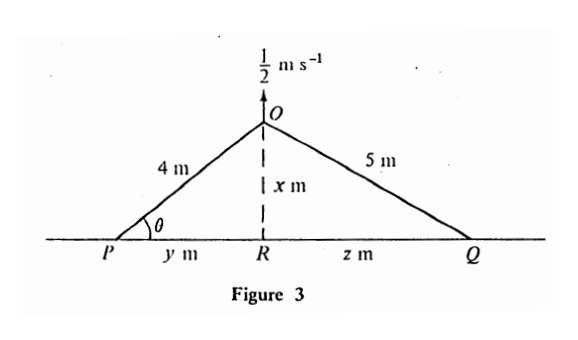
\includegraphics[scale=1.4]{1994CE_A_MATH_1_12.png}
        \end{figure}
        如圖3,$OP$ 和 $OQ$ 為兩條懸挂在 $O$的鐵棒。 $OP$及$OQ$的長度分別爲 4 m 及 5 m 。末端 $O$ 正以 $\dfrac{1}{2}$ ms$^{-1}$ 的速度垂直移動,並使得末端 $P$ 和$Q$在水平綫上移動。 $R$為 $O$ 在水平綫上的投影。在$t$ 秒時, $OR = x$ m 及 $\angle OPQ=\theta$ ,其中$0<\theta<\dfrac{\pi}{2}$。\begin{enumerate}
            \item \begin{enumerate}
                \item 試以$\theta$表示 $x$。 
                \item 由此,求 $\dfrac{d\theta}{dt}$,并以$\theta$表示。
            \end{enumerate}
            \item 設$PR=y$ m,$RQ=z$ m。\begin{enumerate}
                \item 試以$\theta$表示 $\dfrac{dy}{dt}$及$\dfrac{dz}{dt}$。
                \item 由此,求 $\dfrac{d PQ}{dt}|_{\theta=\pi/6}$。答案取整至3位有效數字。
            \end{enumerate}
            \item \begin{enumerate}
                \item 求 $\theta$的值使得$\triangle OPR$的面積最大化。
                \item 考慮 $\angle OQR$的值,求 $\theta$的值使得$\triangle ORQ$ 的面積最大化。答案取整至3位有效數字。
            \end{enumerate} 
        \end{enumerate}\hfill(23分)

        \hrulefill
            
            \hrulefill
            
            \hrulefill
            
            \hrulefill
            
            \hrulefill
            
            \hrulefill
            
            \hrulefill
            
            \hrulefill
            
            \hrulefill
            
            \hrulefill
            
            \hrulefill
            
            \hrulefill
            
            \hrulefill

            \hrulefill
            
            \hrulefill
            
            \hrulefill
            
            \hrulefill
            
            \hrulefill
            
            \hrulefill
            
            \hrulefill
            
            \hrulefill
            
            \hrulefill
            
            \hrulefill

            \hrulefill
            
            \hrulefill
            
            \hrulefill
            
            \hrulefill
            
            \hrulefill
            
            \hrulefill
            
            \hrulefill
            
            \hrulefill
            
            \hrulefill
            
            \hrulefill
            
            \hrulefill
            
            \hrulefill
            
            \hrulefill

            \hrulefill
            
            \hrulefill
            
            \hrulefill
            
            \hrulefill
            
            \hrulefill
            
            \hrulefill
            
            \hrulefill
            
            \hrulefill
            
            \hrulefill
            
            \hrulefill

            \hrulefill
            
            \hrulefill
            
            \hrulefill
            
            \hrulefill
            
            \hrulefill
            
            \hrulefill
            
            \hrulefill
            
            \hrulefill
            
            \hrulefill
            
            \hrulefill
            
            \hrulefill
            
            \hrulefill
            
            \hrulefill

            \hrulefill
            
            \hrulefill
            
            \hrulefill
            
            \hrulefill
            
            \hrulefill
            
            \hrulefill
            
            \hrulefill
            
            \hrulefill
            
            \hrulefill
            
            \hrulefill

            \hrulefill
            
            \hrulefill
            
            \hrulefill
            
            \hrulefill
            
            \hrulefill
            
            \hrulefill
            
            \hrulefill
            
            \hrulefill
            
            \hrulefill
            
            \hrulefill
            
            \hrulefill
            
            \hrulefill
            
            \hrulefill
            
            \hrulefill
            
            \hrulefill

        \pagebreak
    \end{enumerate}
\end{document}